%!TEX root = ../intro.tex
%******************************
%	 Biological noise 
%*****************************

\section{Biology of expression noise} 

\cor{The intrinsic stochasticity of biochemical reactions contributes to a wide distribution of \glspl{mRNA} and proteins across a seemingly homogeneous populations of cells \citep{Elowitz2002}. 
In the scientific litearature, this phenomenon is often referred to as “biological noise” (see \textbf{Box 1})}
All cellular systems are exposed to varying levels of noise and employ strategies to make use of or cope with this source of variation. 
The sources and consequences of biological noise have been studied in an array of viral, prokaryotic and eukaryotic systems \citep{Raj2010, Balazsi2011, Eldar2010}. 
Across these systems the extent of its function remains unclear. 

\begin{Comment}
\hspace{-2.5mm}\textbf{Box 1: Defining biological noise}\label{box1}\\
\small
Biological noise in cell populations \cor{is defined as} stochastic effects on transcription and translation that propagates to form cell-to-cell phenotypic differences. 
To \cor{understand} noise, one needs to distinguish between different sources of cell-to-cell variability in multiple measurable factors. 
On the broadest level, differences between single cells in a population can arise from structured and unstructured sources. 
When capturing cell populations that contain discrete cell states and/or cell types \citep{Paul2015, Ibarra-Soria2018, Rosenberg2018}, measuring cell-specific features results in the detection of non-stochastic but rather correlated (structured) differences between individual cells. 
When the cell population structure is not driven by correlated features (unstructured variation), continuous processes (e.g.~differentiation) can be the dominating source of cell-to-cell phenotypic variability \citep{Dahlin2018}. 
Computational approaches allow the detection of these trajectories (e.g.~via \gls{PCA} or pseudotime inference \citep{Trapnell2014, Angerer2015}). 
Therefore, \cor{my work and work of others \citep{Faure2017, Morgan2018} focus on studying "molecular phenotypic variability", independent of measurement errors, in homogeneous cell populations as proxy for biological noise}. \\

\cor{Classically and specifically in populations of bacteria} \citep{Elowitz2002}, biological noise has broadly been classified into intrinsic and extrinsic noise. 
Intrinsic noise originates from stochastic biochemical effects that directly influence mRNA and protein expression gene-specifically (e.g.~\gls{TF} binding dynamics, see \citep{Swain2002}). 
Extrinsic noise on the other hand introduces co-variation across multiple genes (also in a pathway specific manner \citep{Raser2005}) due to \cor{variations} in cell-specific factors such as stress response, mitochondrial maintenance, amino-acid synthesis \citep{Stewart-Ornstein2012} or cell cycle \citep{Zopf2013}. 
\cor{Within a population of bacteria,} intrinsic noise can therefore be measured as expression differences between co-regulated genes in one cell, while extrinsic noise is measured as co-regulated variance in gene sets across all cells.
\cor{In multicellular systems however, the observed molecular phenotypic variability is a combination of stochastic (noise) and deterministic effects, which are difficult to delineate.}
\end{Comment}

\newpage

When discussing the role of noise in biological systems, it is crucial to differentiate between unicellular systems (prokaryotes, viruses, and yeast) and higher, multicellular eukaryotic systems that show complex signalling events. 
\cor{Furthermore, measuring the stochastic component of biological noise is difficult and requires time-resolved reporter gene read-outs in truly homogeneous cell populations \citep{Elowitz2002}. 
Due to this, the majority of studies presented in this chapter use the observable molecular phenotypic variation in form of single-cell transcriptomic or proteomic read-outs as proxy for biological noise (see \textbf{Box 1}). 
This variation is confounded by unobserved deterministic processes (e.g subtle cell-cycle variation) and delineating the stochastic and deterministic component is challenging.}

\subsection{Bet-hedging in unicellular systems}

Biological noise has been \cor{proposed} to trigger the differential decision between latency and replication in viruses such as \gls{HIV} and the $\lambda$-phage. 
In the case of the $\lambda$-phage, infected cells either reside in a lysogenic state where the genetic material of the virus is transmitted to daughter cells without inducing cell death, or a lytic state where the virus destroys the host cell \textbf{(Fig.~\ref{fig0:bedhedging})} \citep{Lieb1953}. 
Previous studies have shown that the lysis-lysogeny switch in $\lambda$-phage is driven by intrinsic and extrinsic noise \citep{Arkin1998, St-Pierre2008}. 
This idea has been extended by Zeng \textit{el al.}, 2010 where the lysis-lysogeny switch does not depend on a single noise-driven decision but on the sum of all individual phages per cell \citep{Zeng2010}. 
\cor{In general, by summing across stochastic events or if the lysis-lysogeny decision can be predicted based on cellular volume, the switch does not occur as stochastically as initially anticipated.}
In the case of \Gls{HIV}, the virus either rapidly replicates or resides in a long-lived latent state from which the virus can switch to replication \citep{Weinberger2015}. 
It has been shown that combining noise-enhancing and activating drugs shifts latent viruses into the active-replication state that can be targeted by anti-retroviral therapeutics \citep{Dar2014}. 
\cor{Independent of the stochastic contribution to the latency-replication switch, this study present one of the first approaches to modulate phenotypic variability of a biological system to enhance therapeutic efficiency.}\\

In unicellular organisms, \cor{biological noise has been linked to ‘bet-hedging’ strategies, where a sub-optimal fitness landscape is tolerated across a population of cells in order to facilitate an effective response to environmental changes.} Here, phenotypic heterogeneity facilitates the commitment to alternative cell states in cases of stress (e.g.~nutrient deprivation, temperature fluctuations). 
For example, \Gls{Bsubtilis} either commits to sporulation or competence upon starvation or DNA damage. 
Sporulation describes an irreversible process during which vegetative growth ends and the cell forms endospores that survive the altered environment. 
Competent bacteria on the other hand take up DNA from endospores to repair DNA damage \citep{Schultz2009}. 
The probabilistic and transient activation of competence in a sub-population of \Gls{Bsubtilis} cells is modulated by fluctuations in the competence regulators ComK and ComS. 
An excitable system of negative and positive feedback loops controls the number of cells that reversibly commit to competence while other cells irreversibly execute sporulation \citep{Suel2006}. 
\cor{Variations} in the process of transferring phoshporyl groups across a cascade of regulators maintains a constant probability for cells committing to sporulation under nutrient deprived conditions \citep{Russell2017}. 
A similar phenomenon is observed in \Gls{Ecoli} populations exposed to antibiotics where pre-existing phenotypic heterogeneity allows some cells to resist antibiotic treatment. 
Once regrown, these cells remain sensitive to the antibiotic \citep{Balaban2004}. 

\begin{figure}[!h]
\centering
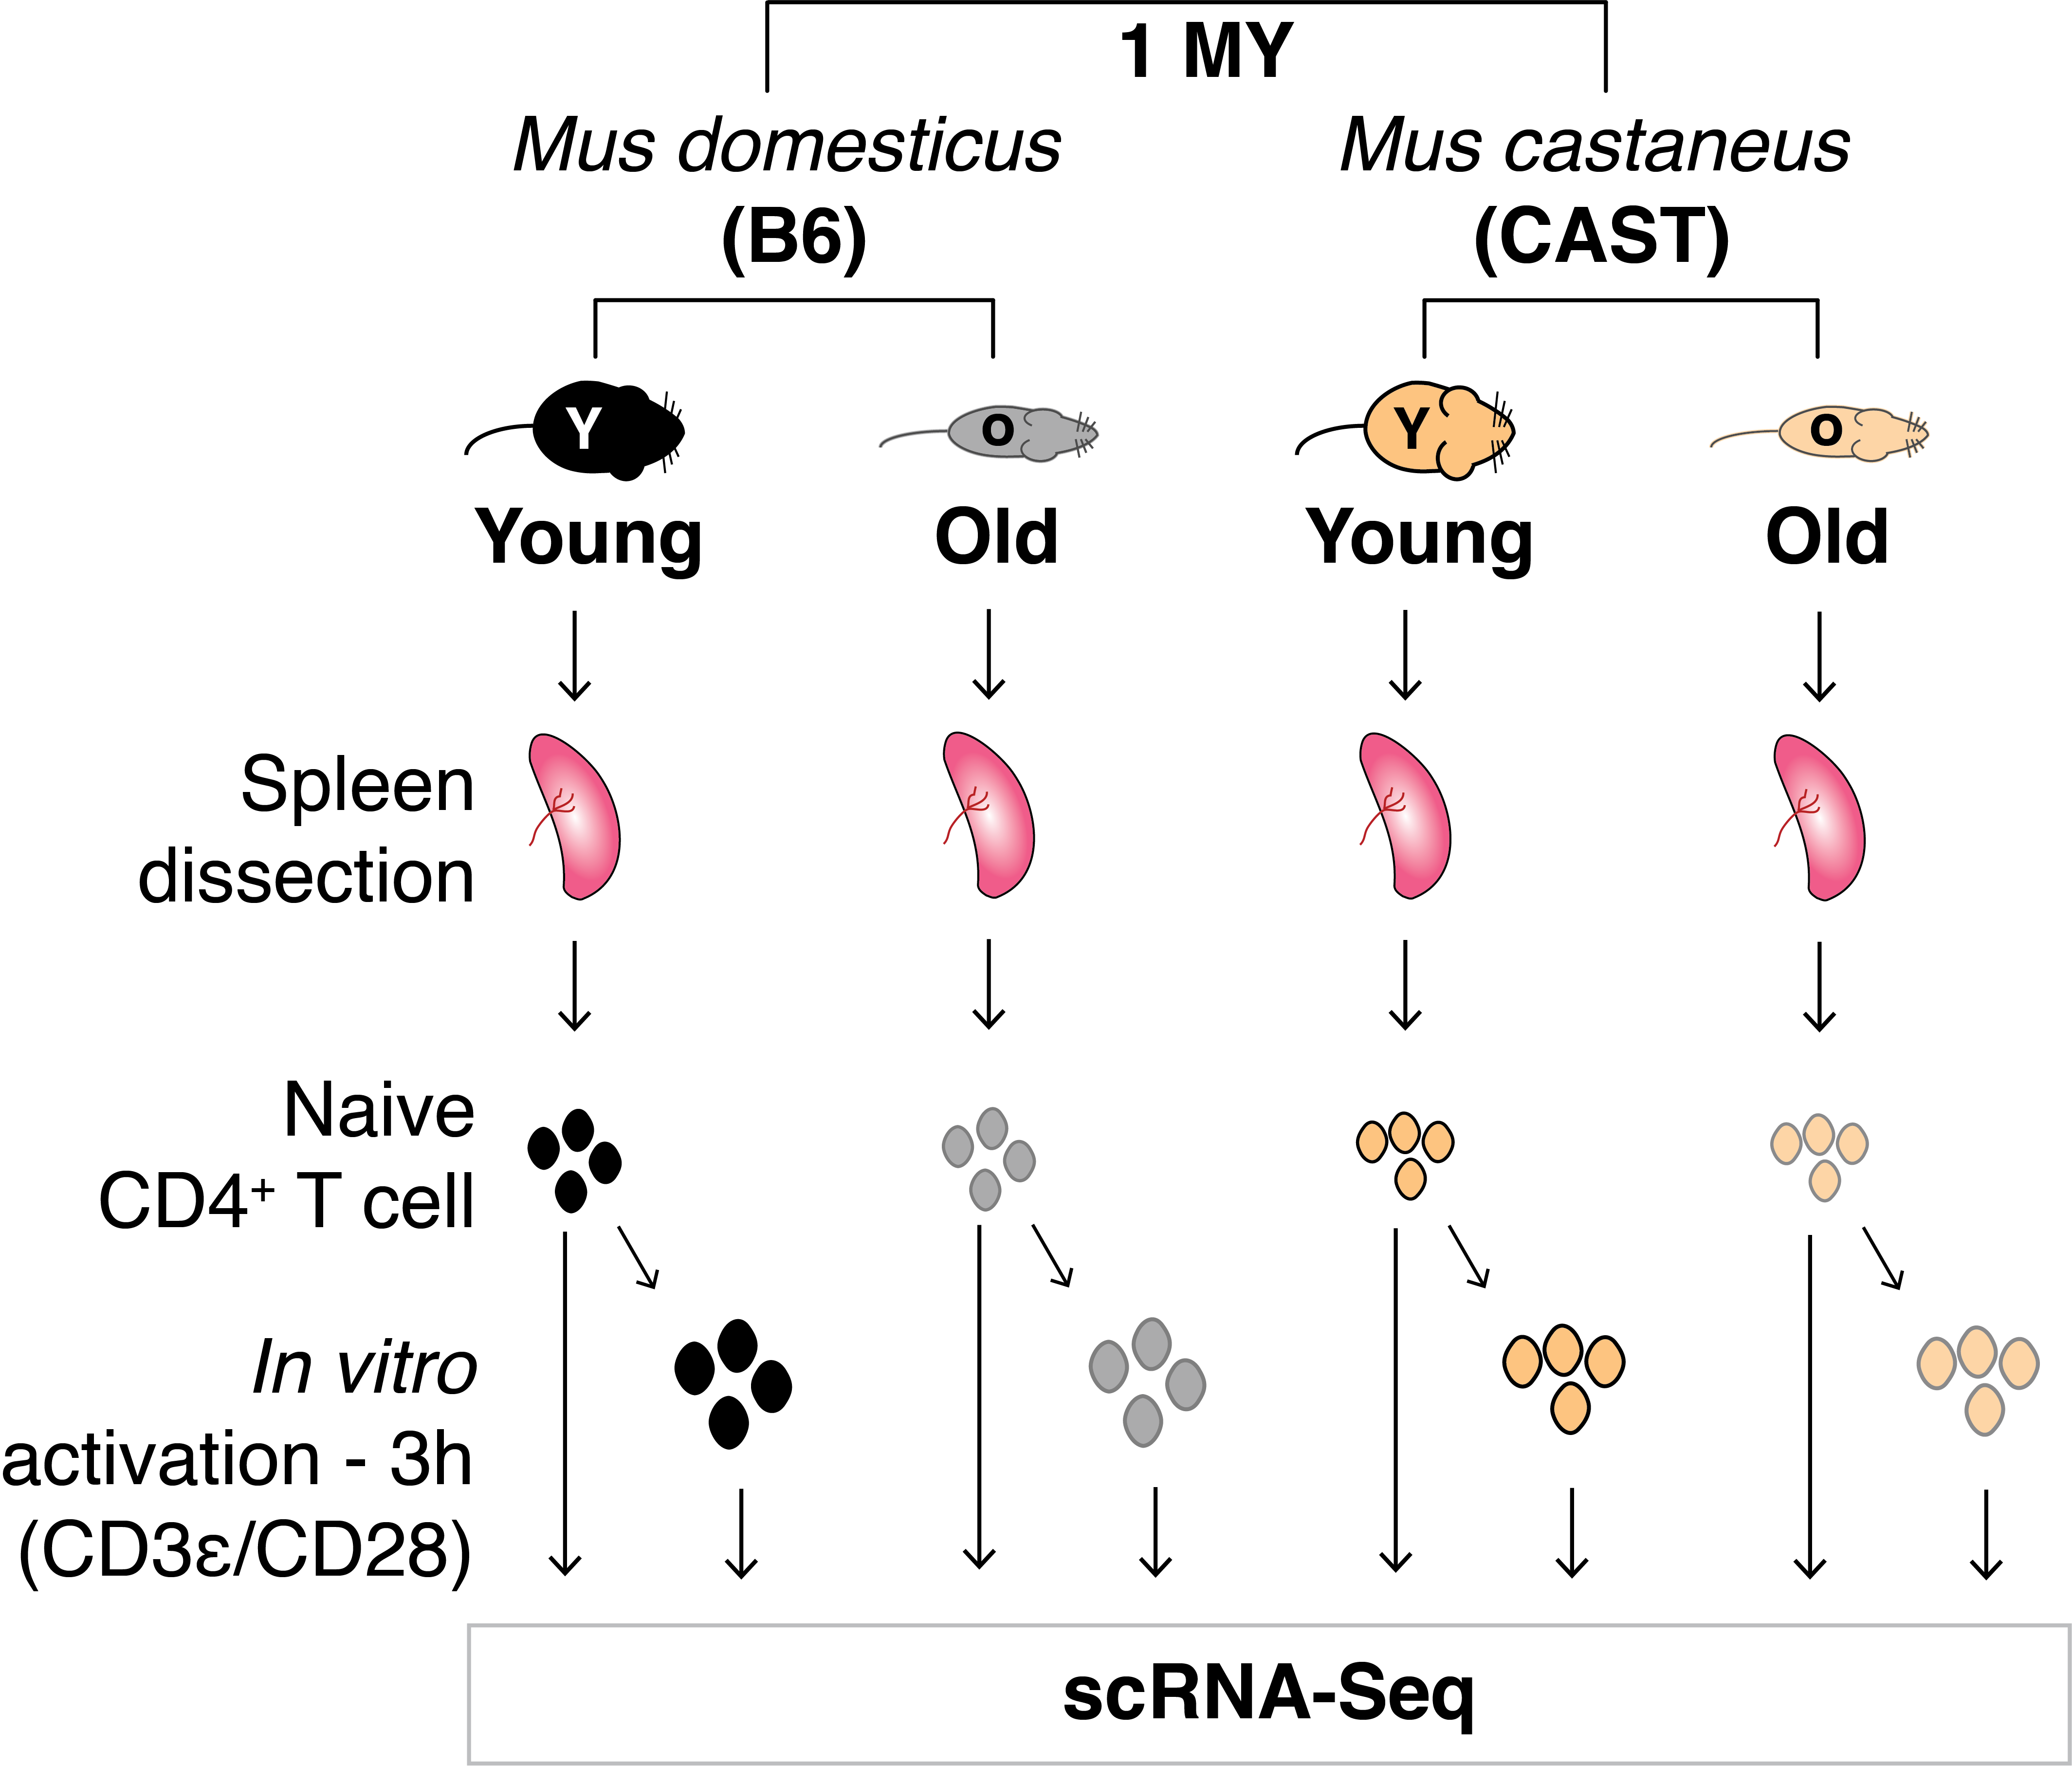
\includegraphics[width=\textwidth]{Fig_1.png}
\caption[Bet-hedging strategy of the $\lambda$-phage]{\textbf{Bet-hedging strategy of the $\lambda$-phage.}\\
The linear genome of the $\lambda$-phage enters the \Gls{Ecoli} host cell and circularises. 
A stochastic decision is made to enter the (i) lytic or (ii) lysogenic cycle where (i) the $\lambda$-phage genome replicates, the $\lambda$-phage particles assemble in the host cell and the cell is destroyed releasing the virions or (ii) the $\lambda$-phage is integrated into the host genome (prophage) and transferred to daughter cells during cell divisions. 
Under stress conditions, the $\lambda$-phage genome is excised from the host genome and enters the lytic cycle.}
\label{fig0:bedhedging}
\end{figure}

Similar to phenotypic heterogeneity in unicellular prokaryotes, transcriptional noise facilitates the switching between mating phenotypes in yeast upon exposure to pheromones \citep{Paliwal2007}. 
Comparably, commitment to utilising galactose as a nutrient source is a cell fate transition, which is facilitated by stochastic gene expression \cite{Acar2008}. \\

\cor{In these systems, biological noise introduces variation in mRNA and proteins that increase plasticity for cells to adapt to changeing environments.
However, to control and balance the number of cells that commit to a specific fate, noise needs to be buffered, for example, by the regulatory network of feedback loops controlling sporulation and competence.}

\subsection{Development and differentiation}

Similar to bet-hedging strategies in unicellular organisms, noise can facilitate the switch between cell states and the probabilistic induction of differentiation processes \citep{Eldar2010, Chang2008}.
\cor{However, as mentioned above, measuring biological noise in differentiating multi-cellular organisms is challenging and the observed molecular phenotypic variability is a combination of stochastic and deterministic components.} 
It has been shown that transcriptional \cor{variability} increases throughout differentiation \citep{Stumpf2017} and development \citep{Antolovic2017}. 
Dissecting differentiation processes of haematopoietic progenitor cells revealed an increase in transcriptional \cor{variability} directly before cell fate decisions are made \citep{Mojtahedi2016, Richard2016}. 
Once committed, differentiating cell populations collapse in variability and move towards a new attractor state. 
\cor{These studies highlight a possible contribution of molecular variability to cell fate decision event.
However, the observed change in variability within differentiating cell populations is purely correlative and it is not possible, with these experiments, to differentiate between variability causing differentiation or differentiation causing variability.}\\

Studies of recent years proposed that stochasticity in expression \cor{contributes to} early (pre-implantation) embryonic development, and to gastrulation \citep{Dietrich2007}. 
As early as the 4-cell stage embryo, targets of master pluripotency factors Oct4 and Sox2 are heterogeneously expressed \textbf{(Fig.~\ref{fig0:noise_development}, left panel)}. 
This is caused by heterogeneous methylation patterns of \gls{H3R26} induced by \gls{Carm1}, which in turn facilitates the binding of Oct4 and Sox2 to induce pluripotency. 
Cells with unmethylated H3R26 differentiate towards the extra-embryonic trophoectoderm while pluripotent cells form the inner cell mass \citep{Goolam2016}. 
Once the cells compact at \gls{E} 3.5, cells of the \gls{ICM} stochastically express genes to initiate heterogeneity within the cell population \textbf{(Fig.~\ref{fig0:noise_development}, 2\textsuperscript{nd} panel)}. 
Fgf4 driven signal reinforcement controls this heterogeneity to form a salt-and-pepper like cell state pattern at E3.5. 
Positional information and the establishment of gene regulatory networks facilitate the segregation of the epiblast and primitive endoderm lineage at E4.5 \textbf{(Fig.~\ref{fig0:noise_development}, 3\textsuperscript{rd} panel)} \citep{Ohnishi2014}. 
In line with this, scRNA-Seq revealed high levels of \cor{transcriptional variability} in the uncommitted inner cell mass at E3.5 (64-cell stage) in comparison to the E4.5 committed epiblast. 
\cor{Transcriptional variability} increases again upon exit from pluripotency in the E6.5 epiblast while cells of the primitive streak at E6.5 synchronise their expression patterns and \cor{variability} is reduced \textbf{(Fig.~\ref{fig0:noise_development}, right panel)} \citep{Mohammed2017}. \\

\cor{Besides the hypothesis of transcriptional variation contributing to embryonic development, a number of alternative drivers for cell fate decisions the mouse embryo exist \citep{Zhang2018a}. 
For example, in the 8-cell to 16-cell stage embryo, symmetry breaking could be achieved by an interaction between the cell’s position and polarity, its cortical tension, and the orientation of cell division \citep{Zhang2018a}. 
Maître \emph{et al.} proposed a system where robust self-organization of 8- to 16-cell stage embryos is achieved by differences in contractility between polar and apolar cells, which leads to the internalization of the more contractile apolar cells \citep{Maitre2016}. 
Taken together, it is unclear to which fraction transcriptional variability plays a role in cell fate decision-making and if purely the occurrence of differentiating cells induces transcriptional variation. }

\begin{figure}[!h]
\centering
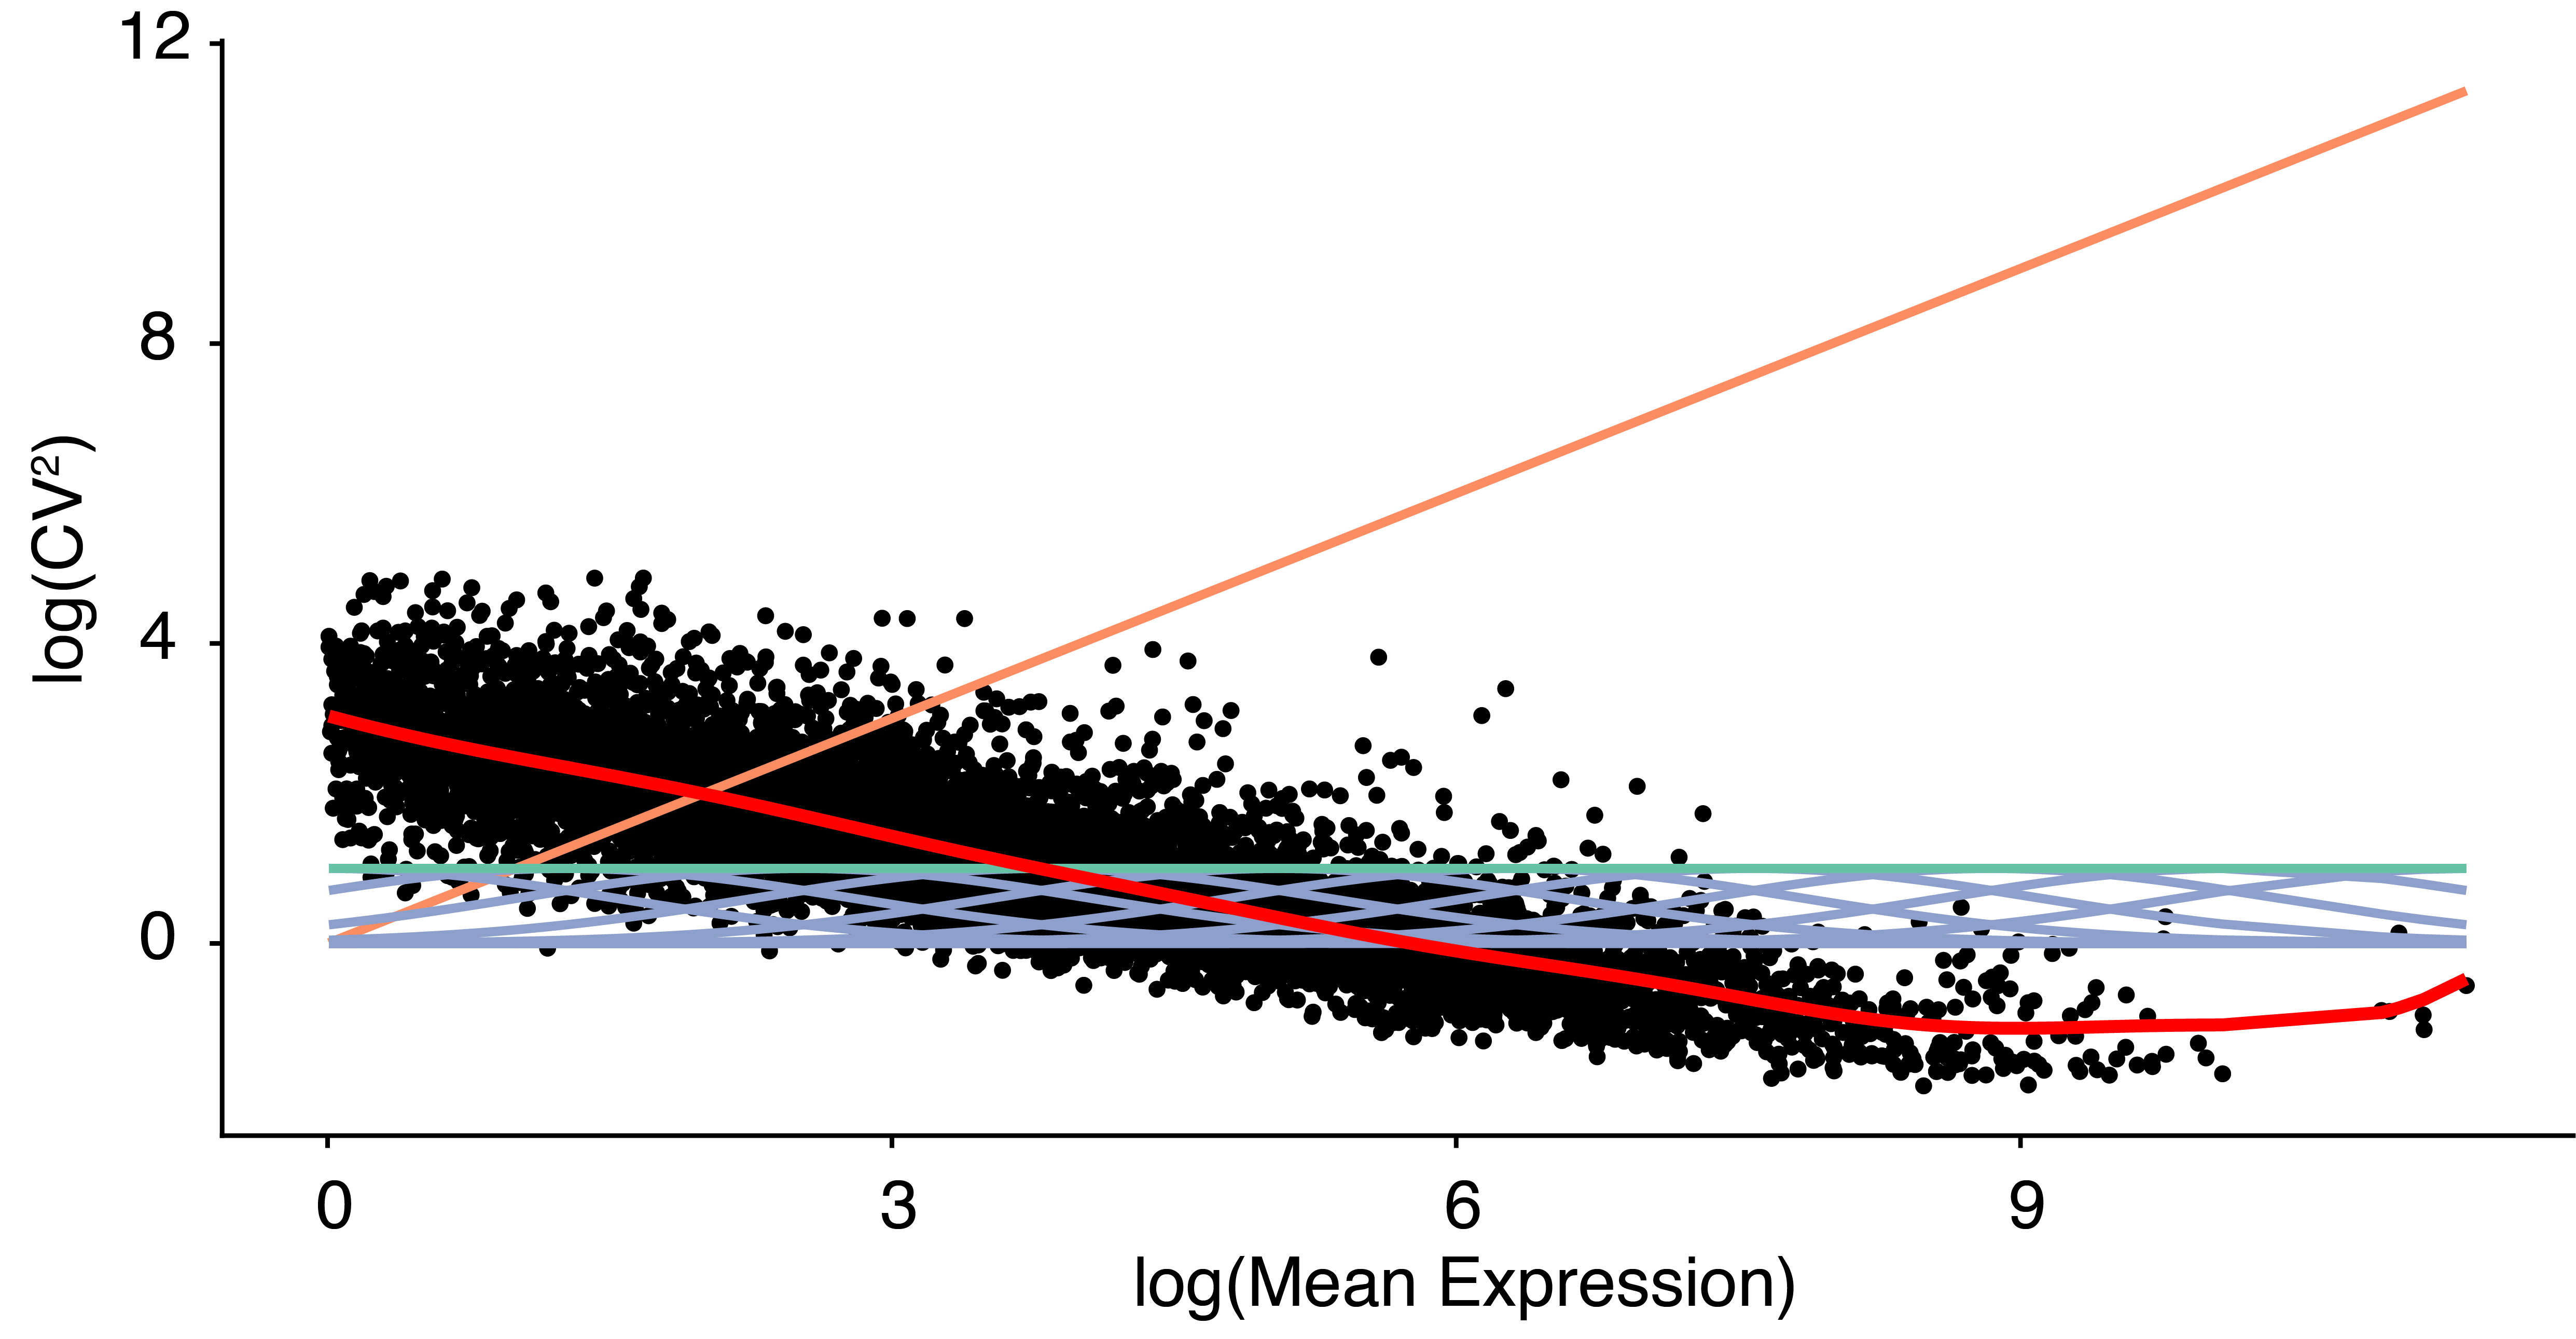
\includegraphics[width=\textwidth]{Fig_2.png}
\caption[Progression of transcriptional heterogeneity during embryonic development]{\textbf{Progression of transcriptional noise during embryonic development}.\\
From left to right: schematic of mouse embryonic development from the 4-cell stage to early gastrulation at E6.5. 
Cell colours indicate gene expression strength. Variable expression at the 4-cell stage induce commitment to form extra-embryonic lineages or pluripotent cells. 
These pluripotent cells at E3.5 show high expression variability forming the inner cell mass (ICM). 
Cells rearrange to form the epiblast and primitive endoderm at E4.5 while noise levels increase in the epiblast at E6.5 compared to the primitive streak.}
\label{fig0:noise_development}
\end{figure}

While pluripotent stem cells in the mouse embryo commit irreversibly to cell lineages during development, \emph{in vitro} cultured \glspl{mESC} reside in a self-renewing, metastable state \citep{Hayashi2008} and heterogenity within the cell population depends on the growth condition. 
Transcription factor heterogeneity, especially of the pluripotency regulator Nanog, is highest in \gls{LIF}/serum grown cells and allows the Nanog-negative cells to commit to differentiation \citep{Chickarmane2012, Torres-Padilla2014}. 
Heterogeneously expressed genes that show a bimodal distribution in expression counts correlate with each other indicative of the presence of distinct states in mESCs. 
These distinct states show differences in promoter methylation patterns, introducing the role of epigenetic modifications to maintain heterogeneity in mESCs \citep{Singer2014}. 
In-depth analysis of mESCs grown in different media (serum, \gls{2i} and \gls{a2i}) shows the presence of three distinct cell states in the serum grown cells. 
mESCs grown in 2i media show less variability in pluripotency markers but higher heterogeneity in cell cycle related genes \citep{Kolodziejczyk2015cell}. 
From the pluripotent ground state, mESCs can differentiate along somatic lineages via specific differentiation events or noise-induced transitions between attractor states. 
Mathematical modelling has shown that mESCs differentiate stochastically through distinct hidden cell (micro-)states within a defined (macro-)state coupled to an increase in variability \cite{Stumpf2017}.
In contrast to the beneficial features of noise in stem cell differentiation, stochastic events during \gls{iPSC} reprogramming limit the formation of single iPSCs \citep{Hanna2009, Yamanaka2009}. 
It has been shown that probabilistic events dominate in an early phase of reprogramming while the transcription of \textit{Sox2} induces a later, more deterministic, phase \cite{Buganim2012}.\\

\cor{These findings indicate an intrinsic heterogeneity of pluripotent cell populations. 
Extrinsic cues, such as growth medium or signalling networks in the embryo, are needed to control this heterogeneity.
However, it is not clear if this seemingly random expression of pluripotent marker genes is truely stochastic or driven by unobserved regulatory mechanisms.
Hoppe \emph{et al.} challenged the idea of lineage choice by stochastic fluctuations of lineage-specific transcription factors and highlighted, using time-resolved measurements, that these transcription factors are solely reinforcing lineage choice \cite{Hoppe2016}.
Therefore, lineage choice can be initiated by unobserved cues that induce variation in genes expression.} 

\subsection{Stochasticity in immune responses}

Fast and flexible immune responses are only possible within cell populations that show high plasticity and react to a broad spectrum of stimuli. 
Stochasticity in cytokine expression \cor{can} lead to phenotypic variability in the \Gls{Th} cell repertoire and increases the effectiveness to respond upon immune stimuli \citep{Schrom2017}. 
For example, fluctuating expression of the lineage defining cytokines \gls{Ifn}\textgamma{} for Th1 and \gls{Il} 4 for Th2 in small populations of cells drive the cell population towards a Th1 or Th2 cell fate while most cells co-express the lineage defining transcription factors \Gls{Gata} 3 and \Gls{Tbx21} \citep{Fang2013a, Antebi2013}.\\

Furthermore, Shalek \textit{et al.}, 2014 have shown that upon \gls{LPS} stimulation a small subset of dendritic cells become activated much earlier than the rest of the cell population while expressing \gls{Ifn}\textbeta. 
These early responders support the activation of late responding cells via cell-to-cell communication (paracrine signalling) and self-stimulation via autocrine signalling \textbf{(Fig.~\ref{fig0:noise_immune})} \citep{Shalek2014}. 
Likewise, a bimodal (digital) expression of Il2 is detected in \gls{Th} cells after immunisation where the number of Il2 expressing cells scales with antigen level. 
Il2 expressing cells support the activation of surrounding cells via paracrine signalling \citep{Fuhrmann2016}. 
Similarly, digital activation processes can be observed in the \gls{NFkB} signalling pathway. 
The fraction of cells that activate this signalling pathway increase with LPS concentration to avoid strong immune activation at low concentrations of a stimulus \citep{Kellogg2015b}. 

\begin{figure}[!h]
\centering
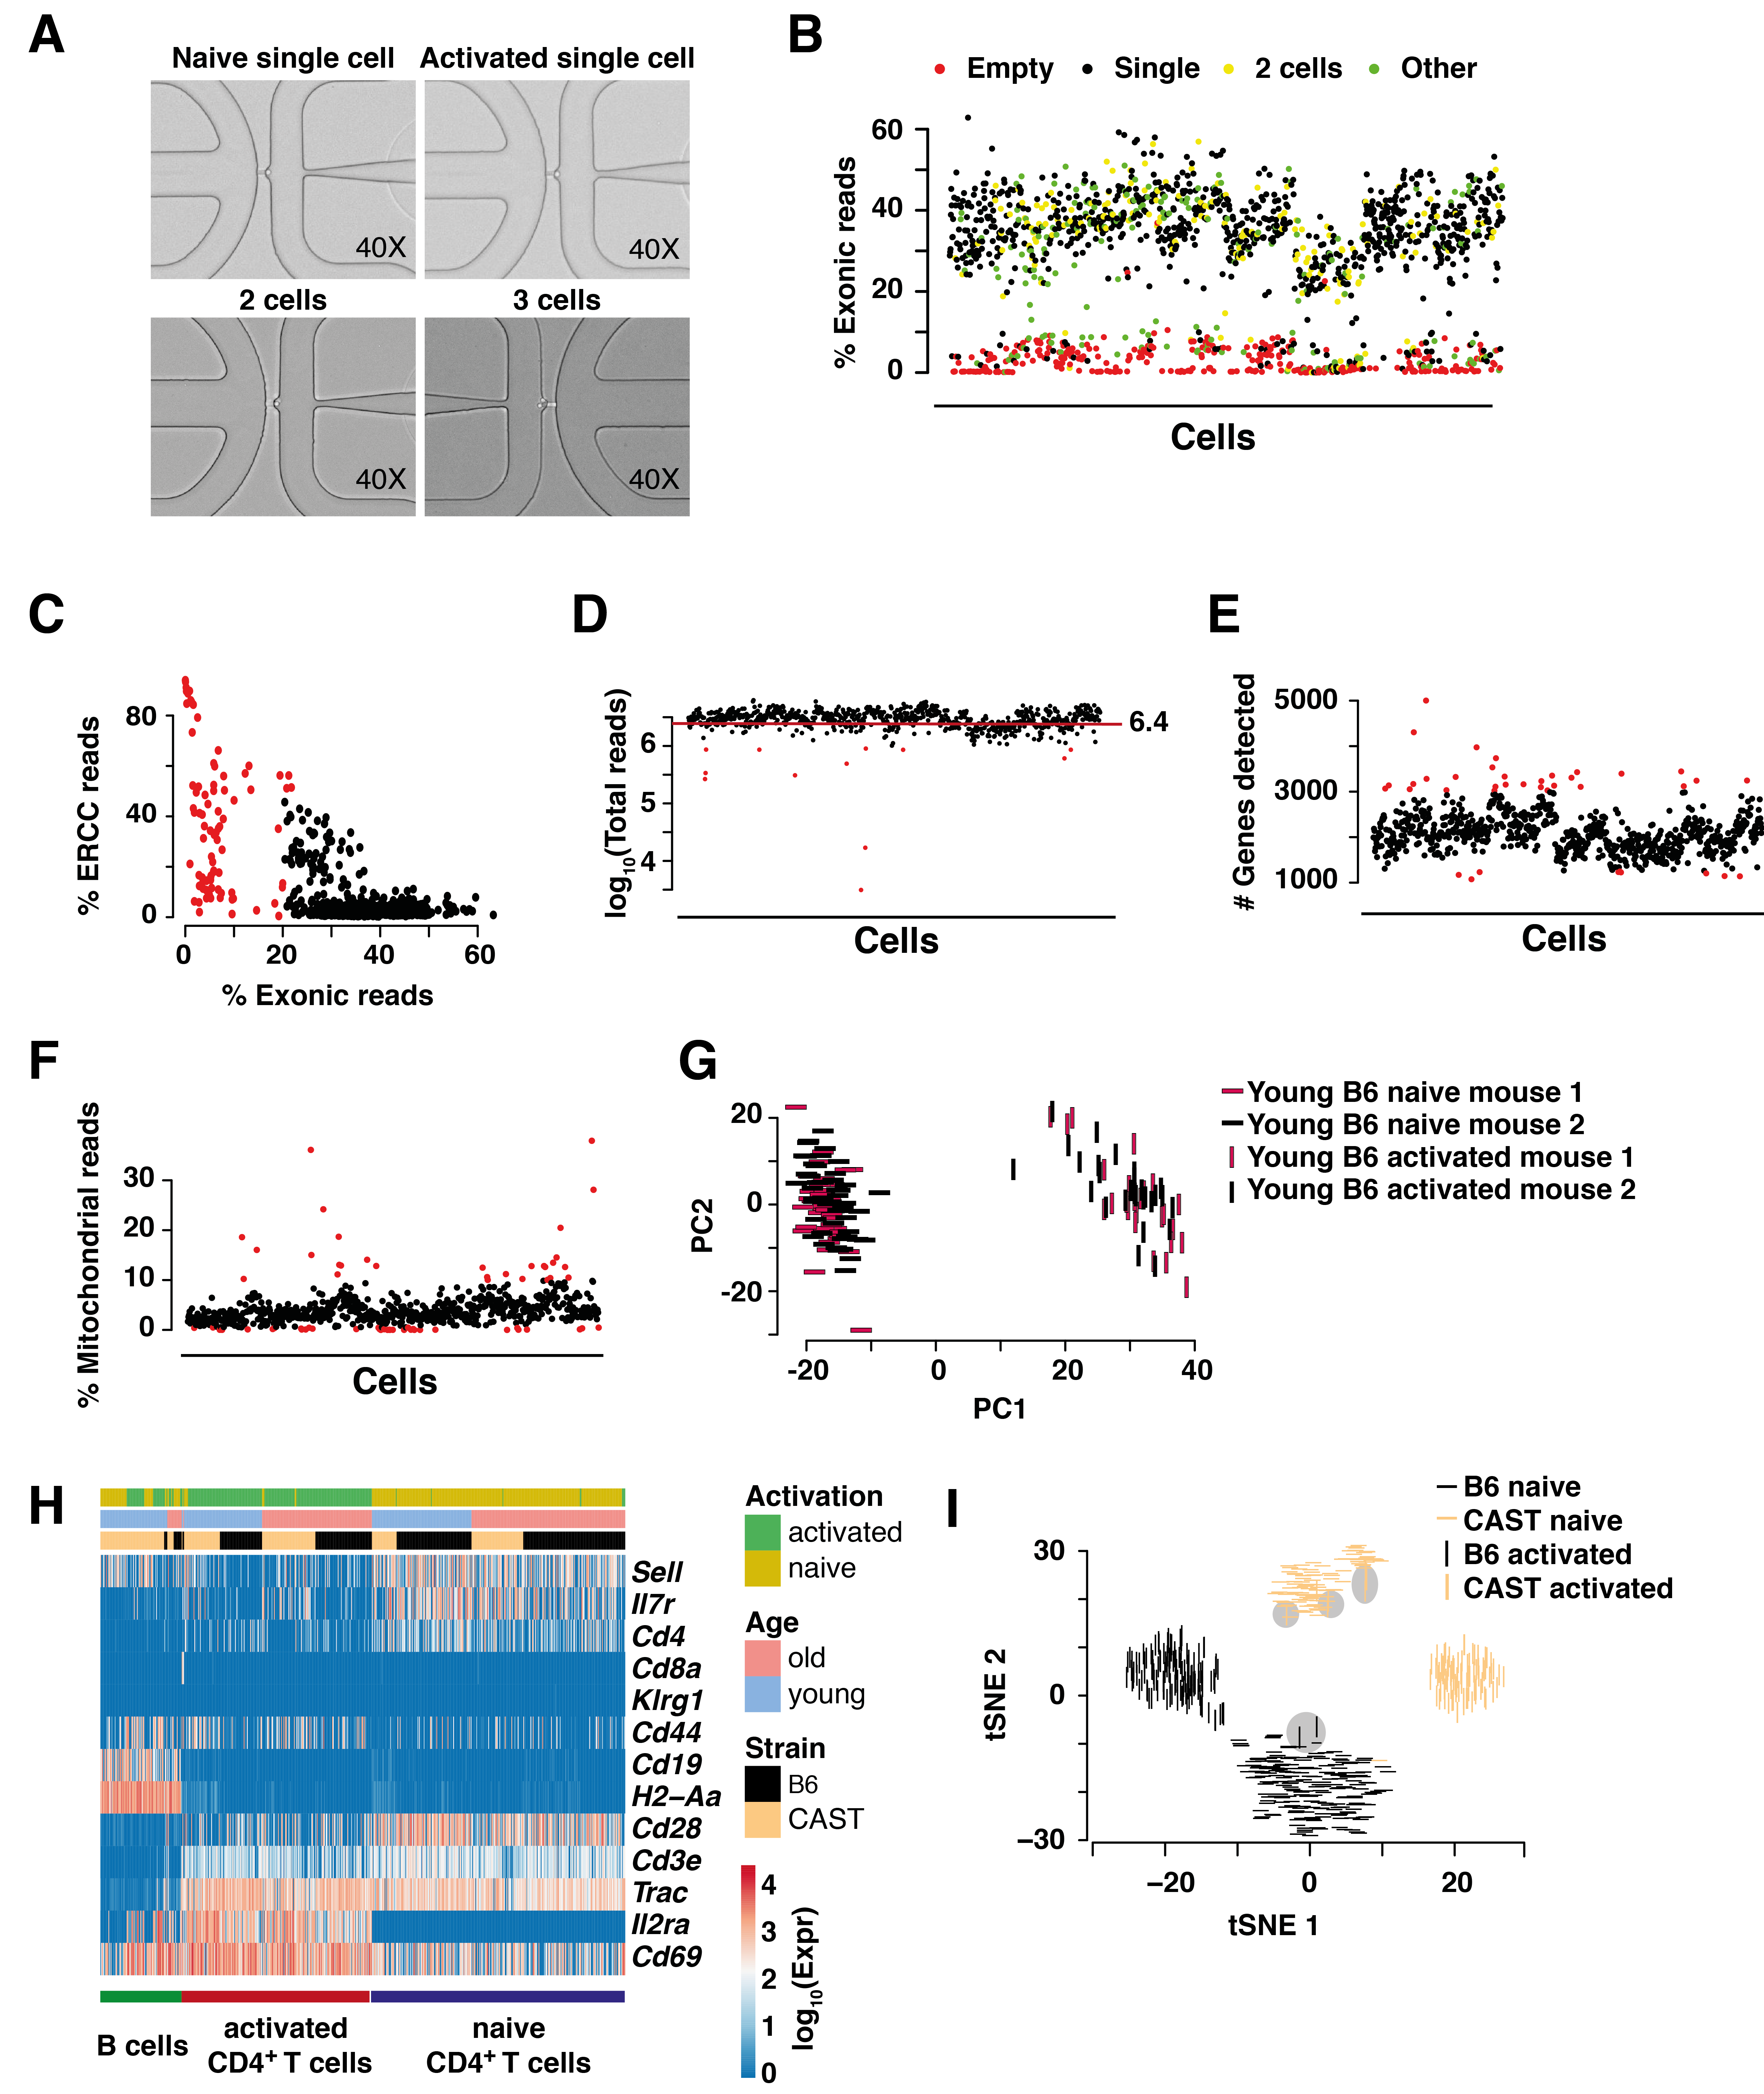
\includegraphics[width=\textwidth]{Fig_3.png}
\caption[Early responders are important for homogeneous immune activation]{\textbf{Early responders are important for homogeneous immune activation.}\\
Within a population of immune cells (e.g.~\gls{DC}, \gls{Th} cells), a sub-population either show higher response strength or induce the production of cytokines such as \gls{Il}2 or \gls{Ifn}\textbeta. 
These early responders induce activation of surrounding cells via paracrine signalling and self-stimulation via autocrine signalling.}
\label{fig0:noise_immune}
\end{figure}

\cor{While the plasticity and reactivity of immune cell populations is finely tuned by introducing phenotypic heterogeneity, it is not understood how individual cells commit to each phenotype. 
In part, stochastic expression introduces molecular phenotypic variability that in turn is tightly controlled by external and internal signalling networks. 
It will therefore be crucial to study the behaviour of immune cells while incorporating their spatial location which might allow the prediction of each cell's phenotype \cite{Battich2015}.}

\subsection{Tissue development and homeostasis}

Coping with the influence of biological noise is important for regulated tissue development and homeostasis. 
An early study showed that in order to minimise the effect of stochasticity in development, plants express heat-shock protein 90 to stabilise regulators of growth and development \citep{Queitsch2002}. 
Furthermore, redundancy in the \Gls{Celegans} intestinal gene regulatory network buffers variability in the down-stream master regulator \textit{elt-2}. 
Once highly connected regulators of this network are removed, phenotypic variation arises from bimodal expression of \textit{elt-2} \citep{Raj2010}. 
The cooperation of positive and negative feedback loops in these highly connected regulatory networks ensure robust expression of key developmental genes \citep{Ji2013}. 
Other models have been proposed in which noise helps to form sharp boundaries between neighbouring domains \citep{Zhang2012}. 
Contact based adhesion and repulsion between cells sharpens narrow transition regions by sorting cells within a tissue across small scales. 
Noise-driven cell state plasticity on the other hand allows cells to switch states and therefore helps narrow a wider transition region \citep{Wang2017}. 
The plasticity to migrate within a population of cells also allow the correction of sensing errors. 
These errors are induced by either too strong or too weak responses of individual cells to a signalling gradient \citep{Camley2017}.

\begin{figure}[!h]
\centering
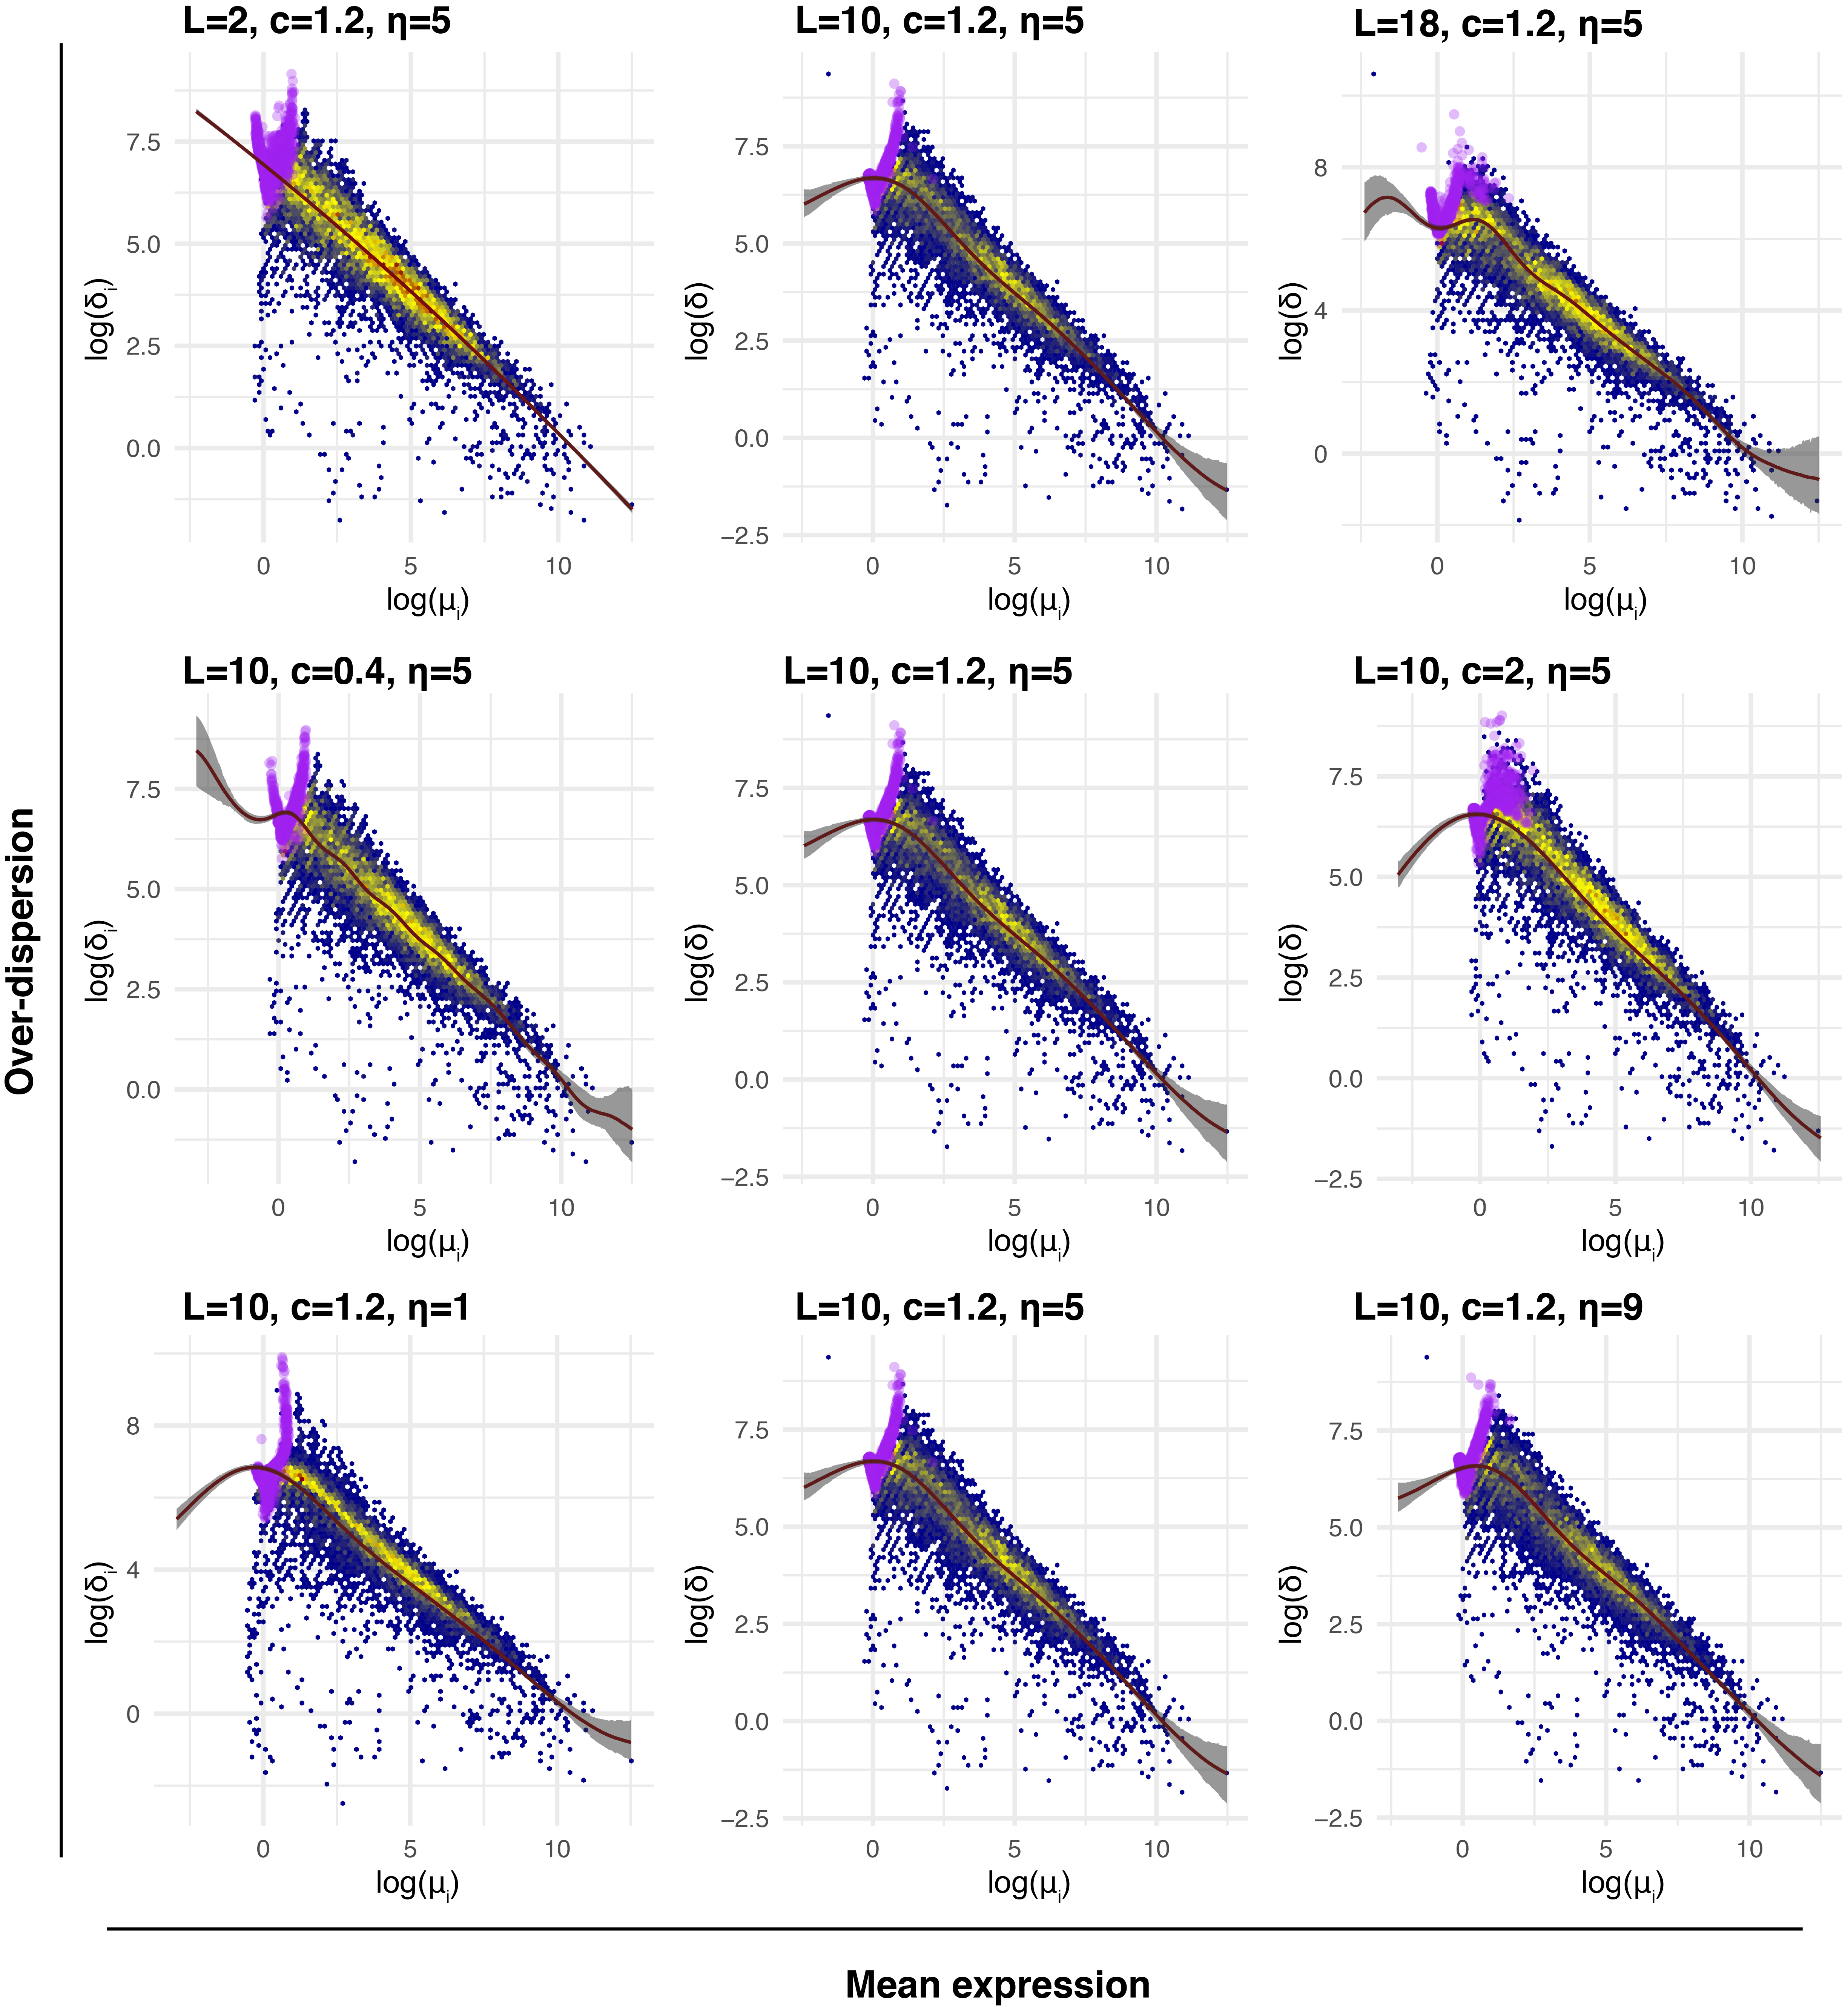
\includegraphics[width=\textwidth]{Fig_4.png}
\caption[Buffering of noise in the colonic crypt]{\textbf{Buffering of noise in the colonic crypt.}\\
Each colonic crypt harbours 6-8 stem cells that divide to form stem cells and progenitors cells. 
Early commitment of progenitor cells to cell fates (e.g.~goblet cells or enterocytes) leads to crypt-to-crypt heterogeneity due to commitment noise (left panel). 
Lateral inhibition within a restricted zone (commitment zone) allows cell fate switching and therefore buffers the crypt-to-crypt heterogeneity (middle panel). 
Migration of goblet cells after the commitment zone buffers the stochastic occurrence of goblet cell or enteroctye patches within the crypt and allows a constant ratio of 1:3 goblet cells to enterocytes in each crypt (right panel). 
Adapted from \citep{Toth2017}.}
\label{fig0:noise_tissue}
\end{figure}

While the cell division rate within tissues is higher during development, tissue homeostasis is maintained by stochastic events that balance cell division and apoptosis \citep{Ranft2010}. 
The effect of noise on maintaining tissue homeostasis has been studied in a diverse set of organs. 
In fat tissue, a complex system of signalling feedback loops controls protein abundance noise to induce differentiation at a low rate but prevents stochastic de-differentiation \citep{Ahrends2014}. 
To maintain coordination in liver function, longer mRNA lifetimes of bursty genes and polyploidy reduce noise in gene expression \citep{BaharHalpern2015}. 
Another mechanism to achieve tissue-wide expression responses involves spatial coordination of stochastically expressing cells in the pituitary gland \citep{Featherstone2016}. 
Spatially constrained signalling events have also been demonstrated to play a role in maintaining colonic crypt cell type diversity. 
Per crypt, eight stem cells differentiate into a defined ratio of cell types. To reduce noise in this process, lateral inhibition within a commitment zone reduces the number of differentiated goblet cells and following slower dispersive migration as well as decreased division rates of goblet cells ensures a distinct 1:3 ratio to enterocytes across all crypts \textbf{(Fig.~\ref{fig0:noise_tissue})} \citep{Toth2017}.\\

\cor{In sum, phenotypic heterogeneity in tissues can arise from stochastic expression driven by noise.
To control for correct tissue responses, signalling networks are in place to modulate this variation. 
In most studies, individual signalling networks and few molecular read-outs were chosen to understand the variation observed within tissues.
However, a combination of multiple regulatory signalling events control cell fate within tissues and disentangling the individual components has not been feasible.}

\subsection{Evolution}

As discussed above, biological noise \cor{can be} beneficial for cell fate commitment \cor{but} needs to be \cor{controlled} to allow coordinated expression in cell populations. 
During evolution, a trade-off between cellular plasticity, the expression responsiveness during environmental changes, and robust expression formed. 
Natural selection acts on genetically controlled expansions of quantitative phenotypes, which\cor{, in part, are} derived from biological noise \citep{Eldar2010}. 
For example, \cor{variable} expression of stress response genes allows a cell population to adapt to changing environments \citep{Lopez-Maury2009}. 
Specifically, the expression of genes controlled by TATA-box containing promoters shows strong divergence between species \citep{Tirosh2006}. 
To control for robust expression levels once selection becomes stabilising, noise levels are reduced \citep{Lopez-Maury2009, Eldar2010, Pires2016}. \\

Lehner, 2008 discussed specifically evolutionary selection to minimise noise in genes that show harmful phenotypic effects upon alteration ("dosage-sensitive genes"). 
These genes show low expression \cor{variability} to reduce the probability of altered expression and also lower expression divergence between species \citep{Lehner2008}. 
Furthermore, essential genes tend to cluster in the genome in regions with persistent open chromatin to reduce \cor{the effect of} noise \citep{Batada2007}. 
In line with this, the promoters of core cellular components show a decoupling between expression plasticity and expression \cor{variability}, which indicates that responsiveness in expression is not a general attribute of high expression \cor{variability} \citep{Lehner2010a}. \\

In unicellular populations, \cor{it has been proposed that the contribution of noise on molecular phenotypic variability} evolutionarily increased as a form of rudimentary regulation \citep{Wolf2015}. 
As a consequence, phenotypic heterogeneity increases the adaption rate of cell populations to extreme environments \cite{Bodi2017}. 
Conversely, in multicellular organisms, collections of cells need to respond in a coordinated manner. 
It has therefore been proposed that nuclear compartmentalisation in higher organisms reduces noise by mRNA retention at the nuclear membrane \citep{Battich2013, Stoeger2016}.\\

\cor{In most cases, cells in an unperturbed state have been profiled to decipher evolutionary selection acting on variability in gene expression.
However, in fluctuating environments where the averaged protein abundance across a cell population is far from the optimum, variability in expression leads to some cells expressing protein levels closer to the optimum. 
By contrast, in stable environments, noise in gene expression can be deleterious by leading to suboptimal growth conditions for many cells \cite{Schmiedel2018,Duveau2018}.
It is therefore crucial to discuss the fitness effect of changes in molecular variability in the context of fluctuating as well as stable environments.}

\subsection{Cancer}

While biological noise \cor{can contribute to} the adjustment of cells to new microenvironments, errors in the form of gene mutations induce transitions from healthy cells towards a cancer attractor state \textbf{(Fig.~\ref{fig0:cancer})} \citep{Marusyk2012}. 
Non-genetic heterogeneity supports the phenotypic adaptation to the new attractor state \citep{Jia2017}. 
The emergence of non-genetic heterogeneity in tumours is coupled to epigenetic dysregulation that allows the survival of cancer cells \citep{Timp2013}. 
Furthermore, it has been proposed that genome wide intra-sample methylation heterogeneity is increased in chronic lymphoitic leukemia increasing cancer cell plasticity in the search for new attractor states \citep{Landau2014}. 
Increased variability in expression can also be observed for more aggressive cancer sub-types across multiple patients \citep{Ecker2015}. \\

An important consequence of \cor{increased} phenotypic heterogeneity in cancer cells is the fractional killing of cell populations upon drug treatment \textbf{(Fig.~\ref{fig0:cancer})} \citep{Flusberg2015}. 
\cor{Variability} in proteins mediating \Gls{TRAIL} induced apoptosis leads to the survival of small fractions of cells \citep{Spencer2009}, which could consequently repopulate the tumour environment. 
Similarly, the stochastic acquisition of DNA damage upon cisplatin exposure introduces heterogeneity in the up-regulation of p53. 
Slow up-regulation leads to cell cycle arrest and inhibits apoptosis while only fast up-regulation leads to cell death \citep{Paek2016}. 
In patient derived melanoma cells, sporadic expression of resistance markers forms a rare cell population that grows into resistant colonies after treatment. 
While pre-resistant cells do not display epigenetic marks and are therefore close to the non-resistant ground state, treatment induces large epigenetic reprogramming, forming stable resistant cancer colonies \citep{Shaffer2017}. 
To tackle this problem, combinatorial therapies have been proposed to reduce variability and fractional killing in cancer cell populations \cite{Paek2016, Roux2015}.

\begin{figure}[!h]
\centering
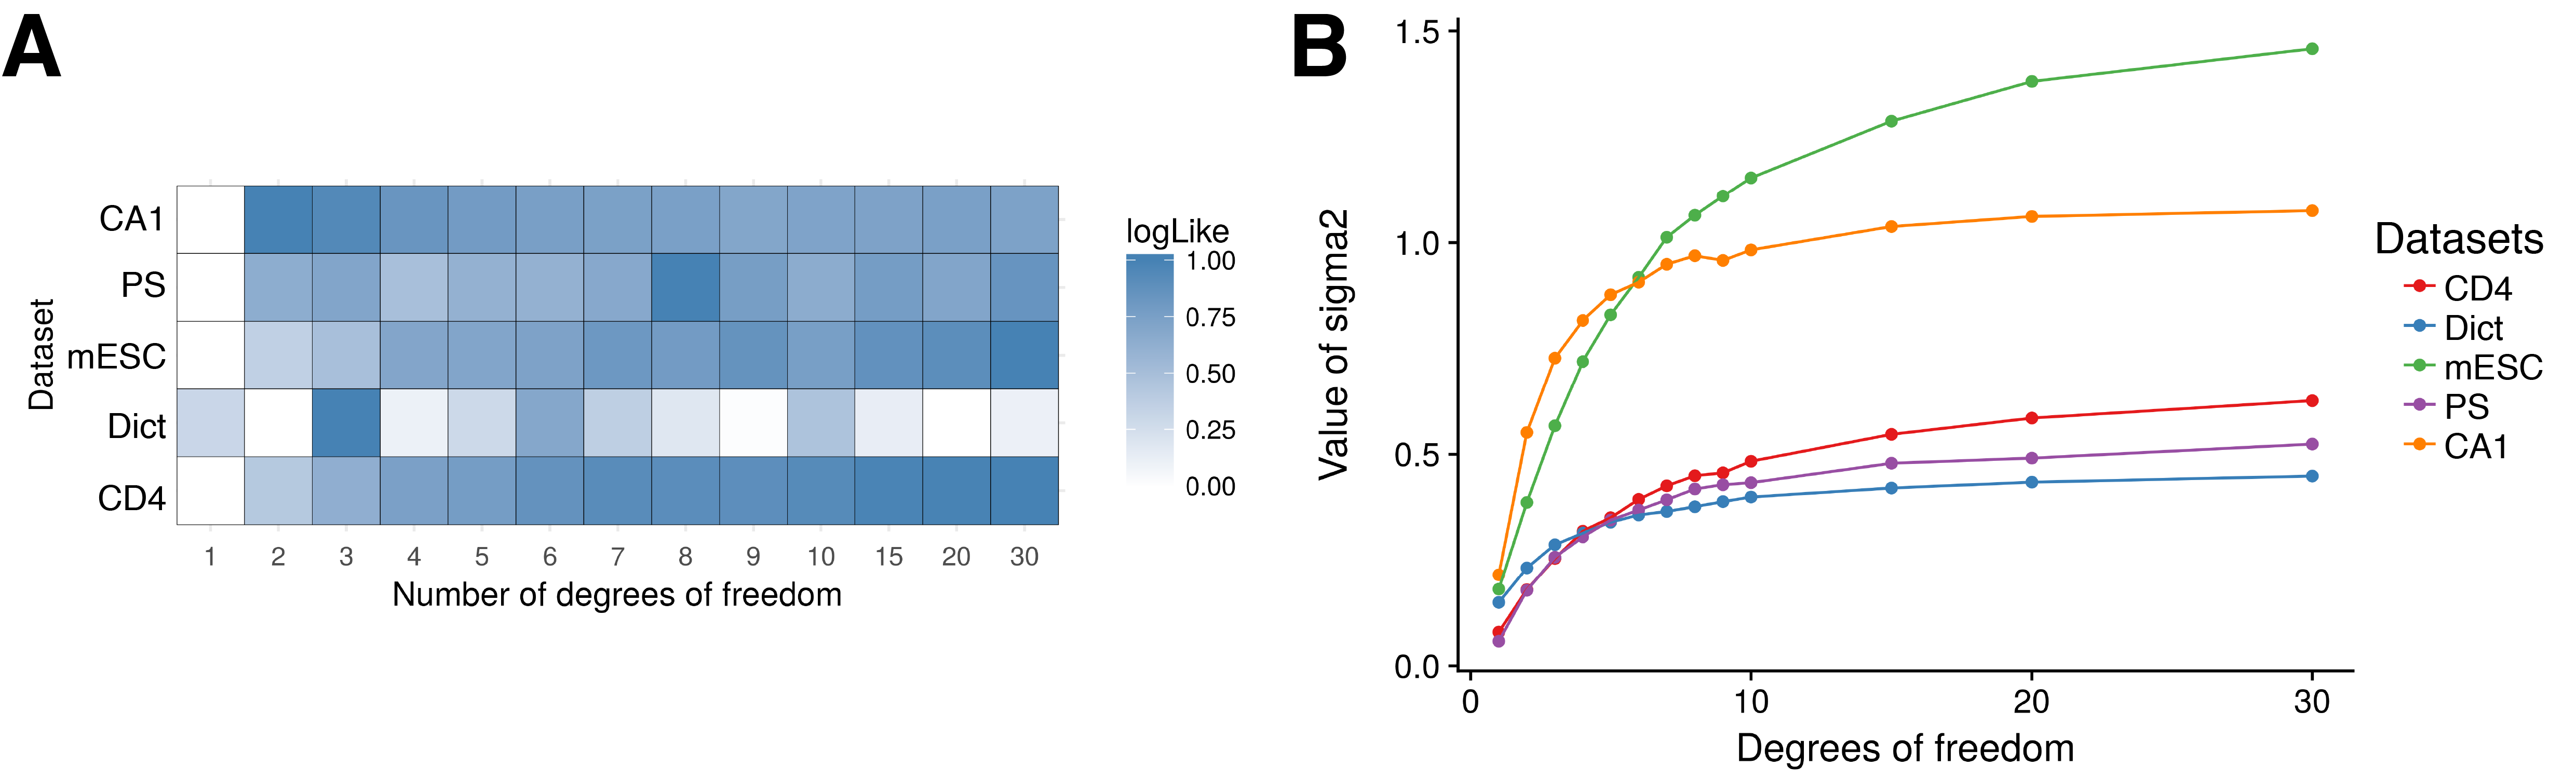
\includegraphics[width=\textwidth]{Fig_5.png}
\caption[Heterogeneous cell states and cell responses in cancer development]{\textbf{Heterogeneous cell states and cell responses in cancer development.}\\
Stochasticity in expression introduces non-genetic heterogeneity that supports the adaptation of cancerous cells. 
Cancer progresses to form a collection of cells with divergent expression patterns. 
This phenotypic heterogeneity leads to fractional killing during treatment and cancer recurrence.}
\label{fig0:cancer}
\end{figure}

\cor{These studies propose a contribution of non-genetic heterogeneity, potentially induced by the loss of noise control, to cancer onset and inefficient treatment response.
However, cancer is a heterogeneous disease that develops in a multi-step process involving disregulation in various cellular systems \cite{Hanahan2011}. 
Therefore, and similar to molecular phenotypic variability in embryonic development, the observed non-genetic heterogeneity can be a phenotypic consequence rather than a driver for cancer onset. }

\subsection{Ageing}

Similarly to the onset of cancer, destructive roles of biological noise have been reported during organismal ageing. 
Previously, it has been debated whether expression noise changes during the lifespan of animals \cite{Bahar2006, Warren2007}. 
While these initial studies only used small panels of genes, transcriptional profiling of single cells led to the discovery of a destabilised immune activation programme in CD4\plus{} T cells due to increased expression noise \cite{Martinez-jimenez2017}. 
Similarly, transcriptional noise increases with age in human pancreas coupled to an increased stress signature and atypical hormone expression \citep{Enge2017}. 
For further discussion of age-related effects on transcriptional noise, see \textbf{Chapter 2}. 

\newpage

\begin{table}[hb	]
\centering
\caption{Positive and negative effects of biological noise on cellular systems.}
\label{table:effects_noise}
\begin{tabular}{l l l}
\toprule
\toprule
\textbf{System} & \textbf{Friend} & \textbf{Foe} \\ 
\midrule
\midrule
Unicellular organism & Bet-hedging & \\
\midrule
Development and & Probabilistic induction  & \\
differentiation & of cell differentiation & \\
\midrule
Immune response & Plasticity in immune response & \\
 & Control of response strength &   \\
\midrule
Tissue development  & Low cell differentiation rate & Non-uniform development \\ 
and homeostasis &  & Uncontrolled tissue response \\
\midrule
Evolution & Adjustment to  & Non-uniform, stabilising expression \\ 
& fluctuating environment & Uncontrolled tissue responses \\
\midrule
Cancer &  & Phenotypic adaption to cancer state \\
& & Fractional killing of cancer cells \\
\midrule
Ageing &  & Unsynchronised immune response \\
& & Increased stress signatures \\ 
\bottomrule
\bottomrule
\end{tabular}
\end{table}
